% File: chapters/chapter3_methodology.tex

\chapter{Methodology and Framework}
\label{chap:methodology}

In this chapter, we explain how the research was carried out, from early experiments to the final deployment at CARIAD SE between May and September 2025. We explain the conceptual foundations of our framework, the technical design that supports it, and the three-phase research strategy that guided our work from initial experiments to enterprise deployment.

The methodology was primarily shaped by the need to rigorously evaluate the application of large language models within complex software security contexts. The research design had to adapt to the rapid advancements in generative AI, where new models and capabilities emerge continuously. Most importantly, the methodology aimed to produce generalizable empirical results that contribute to the broader scientific understanding of automated vulnerability discovery and guide future research directions.

\section{Conceptual Framework: AI-Driven White-Box Fuzzing}
\label{sec:meth_conceptual}

The conceptual framework for this research combines established ideas from software security testing with new possibilities created by large language models. To explain our approach clearly, we first review the core problem and our proposed solution.

\subsection{The Fuzz Driver Problem}
Fuzzing is an effective technique for finding vulnerabilities, but it relies on a critical component: the fuzz driver. A fuzzer like libFuzzer generates raw inputs (byte streams). A fuzz driver is a C++ program that translates those inputs into meaningful API calls to the target library. It acts as the bridge between the random mutations of the fuzzer and the logic of the library.

Writing effective drivers requires deep understanding of the API. An engineer must know what functions exist, what parameters they accept, what preconditions must be satisfied, and what edge cases might cause problems. This understanding represents specialized domain knowledge. Creating effective fuzz drivers requires significant expertise and time, making it a resource-intensive process that is difficult to scale manually against the high volume of modern software production.

\subsection{Our Approach: Automated Generation}
We investigated whether Large Language Models (LLMs) could automate this process. The conceptual idea is straightforward: feed an LLM a description of a target library API (header files, documentation) and ask it to generate a valid fuzz driver.

If the model produces compilable, executable code that achieves meaningful coverage, we have partially automated what previously required human effort. This addresses the bottleneck directly. Instead of assigning a specialist to write each driver manually, we run an automated pipeline, review the output, and deploy it.

We know LLMs have constraints. LLMs sometimes generate code that compiles but does not exercise interesting behavior. They sometimes misunderstand API contracts. They sometimes generate code with undefined behavior that crashes the fuzzer immediately. These are not theoretical concerns; we encountered all of them during our work.

We recognized that imperfect automation still helps. If an LLM generates a driver that achieves 40\% coverage and saves 2 to 8 hours of expert time, that is progress. We do not need perfection. We need a solution that is "good enough" to save time overall.

\section{Technical Architecture Design}
\label{sec:meth_architecture}

Moving from concept to working system required a robust technical design. Our system uses a layered architecture with three main layers: the \textbf{Input Layer}, the \textbf{Generation Layer}, and the \textbf{Execution Layer} (corresponding to Sections~\ref{sec:input_layer}--\ref{sec:exec_layer}). Each layer is marked in Figure~\ref{fig:tech_architecture}.

\begin{figure}[htbp]
    \centering
    \adjustbox{max width=0.95\textwidth, max height=0.75\textheight}{%
    \begin{tikzpicture}[
        databox/.style={draw, rectangle, minimum width=4cm, minimum height=0.9cm, align=center, fill=blue!8, thick, font=\small},
        newdatabox/.style={draw, rectangle, minimum width=4cm, minimum height=0.9cm, align=center, fill=green!15, thick, font=\small},
        procbox/.style={draw, rounded corners=8pt, rectangle, minimum width=4cm, minimum height=0.9cm, align=center, fill=orange!12, thick, font=\small},
        newprocbox/.style={draw, rounded corners=8pt, rectangle, minimum width=4cm, minimum height=0.9cm, align=center, fill=yellow!25, thick, font=\small, draw=orange!80!black},
        arrow/.style={->, >=stealth, thick},
        layerlabel/.style={font=\bfseries\small, rotate=90, anchor=south},
        layerbox/.style={draw, dashed, rounded corners=4pt, inner sep=10pt, fill opacity=0.03}
    ]

    % ============ INPUT LAYER ============
    \node[databox] (srccode) at (0, 0) {Source Code\\{\footnotesize(C/C++ project)}};
    \node[databox] (headers) at (5.5, 0) {Public Header Files\\{\footnotesize(\texttt{.h} / \texttt{.hpp})}};

    \node[newprocbox] (ctxextract) at (2.75, -1.6) {\textbf{Automated Context}\\
    \textbf{Extraction}\\{\footnotesize(cifuzz spark \cite{cifuzzspark})}};

    \node[newdatabox] (apictx) at (2.75, -3.4) {Extracted API Context\\{\footnotesize(signatures, types, classes)}};

    % ============ GENERATION LAYER ============
    \node[newdatabox] (fuzzinstr) at (-2.5, -5.2) {Fuzzing Instructions\\{\footnotesize(libFuzzer harness rules,}\\{\footnotesize safety constraints)}};

    \node[newprocbox] (promptbuild) at (2.75, -5.5) {\textbf{Prompt Construction}\\{\footnotesize(API context + instructions)}};

    \node[newdatabox] (prompt) at (2.75, -7.3) {Assembled Prompt};

    \node[databox] (llmmodel) at (8, -7.3) {LLM Model\\{\footnotesize(local via Ollama /}\\{\footnotesize cloud via Azure OpenAI)}};

    \node[newprocbox] (llmgen) at (5.5, -9) {\textbf{LLM-Based Driver}\\
    \textbf{Generation}};

    \node[newdatabox] (gendriver) at (5.5, -10.7) {Generated Fuzz Driver\\{\footnotesize(C++ source code)}};

    % ============ EXECUTION LAYER ============
    \node[procbox] (compile) at (2.5, -12.3) {\textbf{Compilation}\\{\footnotesize(Clang + ASan/UBSan)}};

    \node[databox] (binary) at (2.5, -13.9) {Instrumented Binary};

    \node[databox] (seedinputs) at (8.5, -13.9) {Seed Inputs};

    \node[procbox] (fuzzexec) at (5.5, -15.5) {\textbf{Fuzzing Execution}\\{\footnotesize(libFuzzer)}};

    \node[databox] (covdata) at (8.5, -17.1) {Coverage Data};
    \node[databox] (crashdata) at (2.5, -17.1) {Crash Reports};

    \node[newprocbox] (coveval) at (8.5, -18.7) {\textbf{Coverage Evaluation}\\{\footnotesize(quality gate)}};

    \node[newdatabox] (covreport) at (8.5, -20.3) {Coverage Report\\{\footnotesize(pass / fail)}};

    % ============ ARROWS ============
    % Input layer
    \draw[arrow] (srccode) -- (ctxextract);
    \draw[arrow] (headers) -- (ctxextract);
    \draw[arrow] (ctxextract) -- (apictx);

    % Generation layer
    \draw[arrow] (apictx) -- (promptbuild);
    \draw[arrow] (fuzzinstr) -- (promptbuild);
    \draw[arrow] (promptbuild) -- (prompt);
    \draw[arrow] (prompt) -- (llmgen);
    \draw[arrow] (llmmodel) -- (llmgen);
    \draw[arrow] (llmgen) -- (gendriver);

    % Execution layer
    \draw[arrow] (gendriver) -- (compile);
    \draw[arrow] (compile) -- (binary);
    \draw[arrow] (binary) -- (fuzzexec);
    \draw[arrow] (seedinputs) -- (fuzzexec);
    \draw[arrow] (fuzzexec) -- (crashdata);
    \draw[arrow] (fuzzexec) -- (covdata);
    \draw[arrow] (covdata) -- (coveval);
    \draw[arrow] (coveval) -- (covreport);

    % ============ LAYER BRACKETS ============
    \begin{scope}[on background layer]
        \node[layerbox, fit=(srccode)(headers)(apictx)(ctxextract), fill=blue!3] (inputlayer) {};
        \node[layerbox, fit=(fuzzinstr)(promptbuild)(prompt)(llmmodel)(llmgen)(gendriver), fill=yellow!3] (genlayer) {};
        \node[layerbox, fit=(compile)(binary)(seedinputs)(fuzzexec)(covdata)(crashdata)(coveval)(covreport), fill=orange!3] (execlayer) {};
    \end{scope}

    \node[layerlabel] at ([xshift=-1.1cm]inputlayer.west) {Input Layer (\S\ref{sec:input_layer})};
    \node[layerlabel] at ([xshift=-1.1cm]genlayer.west) {Generation Layer (\S\ref{sec:gen_layer})};
    \node[layerlabel] at ([xshift=-1.1cm]execlayer.west) {Execution Layer (\S\ref{sec:exec_layer})};

    % ============ LEGEND ============
    \node[databox, minimum width=2.2cm, minimum height=0.55cm, font=\footnotesize] (legdata) at (12, -1) {Data};
    \node[right=0.1cm of legdata, font=\footnotesize] {Existing data};
    \node[newdatabox, minimum width=2.2cm, minimum height=0.55cm, font=\footnotesize] (legnewdata) at (12, -2) {Data};
    \node[right=0.1cm of legnewdata, font=\footnotesize] {New (our contribution)};
    \node[procbox, minimum width=2.2cm, minimum height=0.55cm, font=\footnotesize] (legproc) at (12, -3) {Process};
    \node[right=0.1cm of legproc, font=\footnotesize] {Existing process};
    \node[newprocbox, minimum width=2.2cm, minimum height=0.55cm, font=\footnotesize] (legnewproc) at (12, -4) {Process};
    \node[right=0.1cm of legnewproc, font=\footnotesize] {New (our contribution)};

    \end{tikzpicture}
    }
    \caption{Technical Architecture of our LLM-based fuzz driver generation pipeline. The three layers are marked with dashed borders. Data artifacts are shown in rectangular boxes; processing steps in boxes with rounded corners. Green/yellow highlighted elements denote new contributions of this work with respect to the state of the art (cf.\ Figure~\ref{fig:fuzzing_concept}).}
    \label{fig:tech_architecture}
\end{figure}

As shown in Figure~\ref{fig:tech_architecture}, the source code and its public header files serve as the primary input to the pipeline. These inputs are processed through three successive layers (context extraction, LLM-based generation, and automated execution) to ultimately produce coverage reports and crash data, replacing the manual fuzz driver creation step shown in Figure~\ref{fig:fuzzing_concept}.

\subsection{Input Layer (Automated Context Extraction)}
\label{sec:input_layer}
The first layer prepares the context that the LLM needs to generate a meaningful fuzz driver. Instead of writing custom parsers, we used the analysis capabilities of \textbf{cifuzz spark}, a module of the cifuzz fuzzing toolkit developed by Code Intelligence~\cite{cifuzzspark}. Given a CMake-based C/C++ project, cifuzz spark automatically parses the project structure, identifying public headers and API surfaces relevant for testing. It traverses the abstract syntax tree (AST) to extract function signatures, class definitions, type aliases, and parameter types. The output is the \emph{extracted API context}: a structured summary of the target library's public interface, including function names, their parameter types, return types, and enclosing class or namespace information. This ensures the LLM receives accurate and complete context about the code it needs to test, without requiring manual intervention or maintenance of custom extraction scripts.

\subsection{Generation Layer (LLM Interface)}
\label{sec:gen_layer}
This layer handles the interaction with the LLM and the construction of the prompt that drives driver generation. It includes two critical sub-systems:
\begin{itemize}
    \item \textbf{Prompt Construction:} We combine the \emph{extracted API context} (the structured function signatures, types, and class definitions produced by the Input Layer) with a set of \emph{fuzzing instructions}. These fuzzing instructions are predefined rules and constraints that describe what a valid libFuzzer fuzz driver must look like. Specifically, they define the required \emph{fuzz test case structure}: the driver must implement the \texttt{LLVMFuzzerTestOneInput(const uint8\_t *data, size\_t size)} entry point, correctly consume the fuzzer-provided byte buffer, translate those bytes into valid API calls, and avoid trivial or undefined behavior. The instructions also encode safety constraints (e.g., do not call \texttt{exit()}, avoid infinite loops) to ensure the generated driver is compatible with the fuzzing engine.

    \item \textbf{Backend Abstraction:} We configured the \emph{environment}, that is, the runtime configuration that determines which LLM backend serves the generation requests, to swap between different model backends. While cifuzz manages the overall workflow, we routed the generation requests to both local models (via Ollama) and cloud-hosted models (via Azure OpenAI) to compare performance across different architectures. This abstraction allows the same pipeline to operate in network-isolated environments (using local models) or leverage more powerful cloud models when network access is available.
\end{itemize}

\subsection{Execution Layer (Evaluation Pipeline)}
\label{sec:exec_layer}
The generated fuzz drivers, that is, the C++ source files produced by the LLM in the Generation Layer, are useless if they do not compile and run correctly. This layer handles the automated compilation, execution, and evaluation pipeline:
\begin{enumerate}
    \item \textbf{Compilation and Validation:} The generated driver source code is compiled against the target library using Clang. This step verifies that the LLM-produced code is syntactically valid and links correctly against the target API.
    \item \textbf{Sanitizer Instrumentation:} The driver is recompiled with AddressSanitizer (ASan) and UndefinedBehaviorSanitizer (UBSan) enabled. This detects memory errors, buffer overflows, and undefined behavior that might not cause an immediate crash but indicate incorrect API usage.
    \item \textbf{Fuzzing Execution:} If compilation succeeds, the instrumented binary runs under \texttt{libFuzzer} together with any available seed inputs. The fuzzing engine monitors coverage metrics and records any crashes.
    \item \textbf{Coverage Evaluation:} After the fuzzing run completes, the collected coverage data is evaluated against a quality gate to determine whether the generated driver achieves meaningful coverage of the target library, ensuring the driver is not merely syntactically valid but also behaviorally useful.
\end{enumerate}

\section{Research Strategy: Three-Phase Approach}
\label{sec:meth_strategy}

Our research unfolded in three distinct phases, each addressing different aspects of the research questions defined in Chapter~1.

\subsection{Phase 1: Local LLM Evaluation}
We gathered 14 open-source LLM models ranging from 1.5B to 46.7B parameters and evaluated them on multiple C++ target libraries. This phase directly addresses \textbf{RQ1} and \textbf{RQ2}. Can LLMs generate useful fuzz drivers? Does model size matter? Which models work best?

We chose open-source models specifically because automotive applications have intellectual property constraints. Sending proprietary code to external APIs is often problematic. Local models, run on available hardware, avoid this concern entirely.

\subsection{Phase 2: Model Optimization with LoRA}
Based on Phase 1 results, we selected a promising small model and applied Low Rank Adaptation (LoRA) fine-tuning. We curated a dataset of high-quality fuzz drivers from the Google OSS-Fuzz project to teach the model the specific structure of a good test harness.

The goal was to adapt the model specifically for the fuzzing task while reducing computational cost. This phase addresses \textbf{RQ2} more directly: can smaller, fine-tuned models outperform larger general purpose models?

\subsection{Phase 3: Enterprise CI/CD Integration}
The final phase moved from controlled experiments to the real world. We integrated the solution into CARIAD's actual CI/CD infrastructure. This phase addresses \textbf{RQ3}: Can this approach work in a real corporate environment with real network security policies, cost constraints, and operational complexity?

\begin{figure}[htbp]
    \centering
    \adjustbox{max width=0.95\textwidth, max height=0.55\textheight}{%
    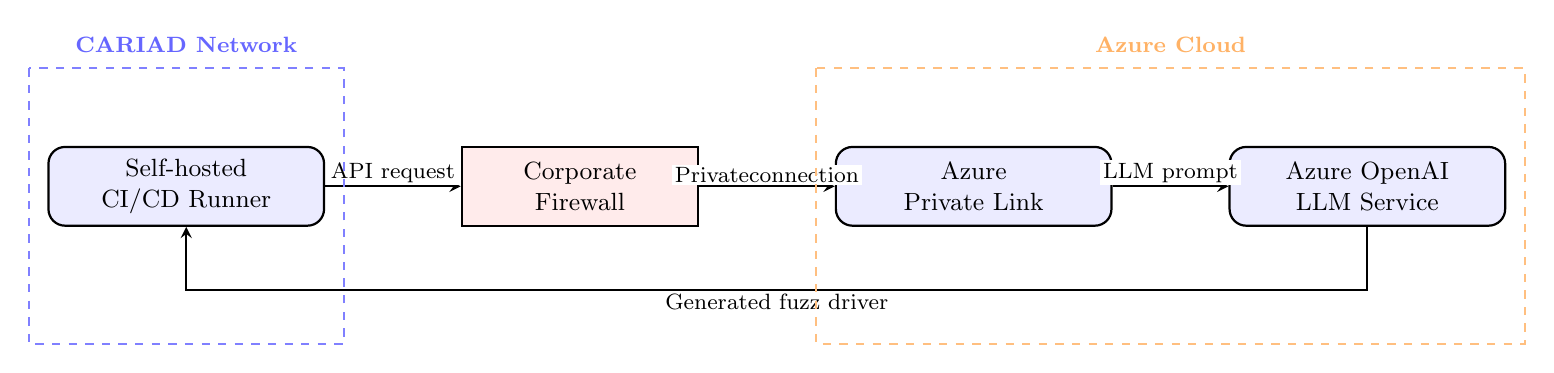
\begin{tikzpicture}[
        comp/.style={draw, rectangle, rounded corners=6pt, minimum width=3.5cm, minimum height=1cm, align=center, fill=blue!8, thick, font=\small},
        datastore/.style={draw, rectangle, minimum width=3.5cm, minimum height=1cm, align=center, fill=green!10, thick, font=\small},
        fw/.style={draw, rectangle, minimum width=3cm, minimum height=1cm, align=center, fill=red!8, thick, font=\small},
        arrow/.style={->, >=stealth, thick},
        blocked/.style={->, >=stealth, thick, dashed, gray},
        edgelabel/.style={font=\footnotesize, fill=white, inner sep=1pt}
    ]

    % --- Corporate side ---
    \node[comp] (runner) at (0, 0) {Self-hosted\\CI/CD Runner};
    \node[fw] (firewall) at (5, 0) {Corporate\\Firewall};

    % --- Azure side ---
    \node[comp] (privatelink) at (10, 0) {Azure\\Private Link};
    \node[comp] (llm) at (15, 0) {Azure OpenAI\\LLM Service};

    % --- Arrows ---
    \draw[arrow] (runner) -- node[edgelabel, above]{API request} (firewall);
    \draw[arrow] (firewall) -- node[edgelabel, above]{Private\\connection} (privatelink);
    \draw[arrow] (privatelink) -- node[edgelabel, above]{LLM prompt} (llm);
    \draw[arrow] (llm.south) -- ++(0,-0.8) -| node[edgelabel, pos=0.25, below]{Generated fuzz driver} (runner.south);

    % --- Boundaries ---
    \draw[thick, dashed, blue!50] (-2, 1.5) rectangle (2, -2);
    \node[font=\footnotesize\bfseries, blue!60] at (0, 1.8) {CARIAD Network};

    \draw[thick, dashed, orange!50] (8, 1.5) rectangle (17, -2);
    \node[font=\footnotesize\bfseries, orange!60] at (12.5, 1.8) {Azure Cloud};

    \end{tikzpicture}
    }
    \caption{Enterprise Integration Strategy. The self-hosted CI/CD runner communicates with Azure OpenAI through a Private Link endpoint, routing traffic through the corporate firewall over a private connection without traversing the public internet.}
    \label{fig:enterprise_integration}
\end{figure}

As illustrated in Figure~\ref{fig:enterprise_integration}, this phase revealed challenges we had not anticipated during earlier work. The corporate firewall blocked external API calls, requiring us to re-architect the solution using Azure Private Link.

\section{Evaluation Methodology}
\label{sec:meth_evaluation}

We evaluated generated fuzz drivers using quantitative metrics to ensure objectivity, focusing on both code quality and pipeline impact.

\begin{itemize}
    \item \textbf{Compilation Success:} Does the driver compile against the target library? This is the first and most critical filter.
    \item \textbf{Runtime Behavior:} Does the driver execute without crashing immediately? We checked if the driver actually runs or just fails instantly.
    \item \textbf{Code Coverage:} What percentage of the target library does the driver test? We measured this using standard tools (\texttt{llvm-cov}).
    \item \textbf{Vulnerability Discovery (MTTV):} We measured the Mean Time To Vulnerability, that is, how long the fuzzer needs to run before it finds a bug.
    \item \textbf{Pipeline Latency (CI Overhead):} We measured how much extra time the AI adds to the build process. The system must stay within CARIAD's CI/CD feedback window (see Chapter~4, Section~\ref{sec:impl_phase3} for the specific performance requirements).
    \item \textbf{Cost and Efficiency:} We calculated the exact price of generating a driver. By tracking the number of tokens (words) sent to the AI, we determined the cost in euros to prove it is cheaper than human engineering.
\end{itemize}

For each target library, we also manually inspected a sample of generated drivers to understand failure modes. We documented cases where drivers compiled but did not work as intended. Finally, we conducted a cost analysis for enterprise deployment, modeling different scenarios to estimate annual expenses.